\documentclass[a4paper,10pt]{article} 


%% Language and font encodings
\usepackage[english]{babel}
\usepackage[utf8x]{inputenc}
\usepackage[T1]{fontenc}

%% Sets page size and margins
\usepackage[a4paper,top=3cm,bottom=2cm,left=3cm,right=3cm,marginparwidth=1.75cm]{geometry}

%% Useful packages
\usepackage{amsmath}
\usepackage{amsmath, amsfonts,xcolor}
\usepackage{amssymb}
\usepackage{xcolor}
\usepackage{amsfonts}
\usepackage{graphicx}
\usepackage{url}
\usepackage[colorinlistoftodos]{todonotes}
\usepackage[colorlinks=true, allcolors=blue]{hyperref}
\usepackage{algorithm}
\usepackage{algpseudocode}

\usepackage{pgfplots}




\newcommand{\marginboxed}[1]{\marginpar{{\large\fbox{#1}}}}
\newcommand {\D}[2]{\frac{d #1}{d #2}}
%
% 2. derivert (total) \Dd{f(t)}{t}
\newcommand {\Dd}[2] {\frac{d^2 #1}{d {#2}^2}}
%
% 1. derivert (partial) \Dp{f(x,y,z,)}{x}
\newcommand {\Dp}[2] {\frac{\partial #1}{\partial #2}}
%
% 2. derivert (partial) \Ddp{f(x,y,z,)}{x}
\newcommand {\Ddp}[2] {\frac{{\partial}^2 #1}{\partial {#2}^2}}
\newcommand {\Ddpp}[2] {\frac{{\partial}^2 #1}{\partial #2^2}}
%
% 1. derivert med index (total) \D{f(t)}{t}{index}
\newcommand {\Dj}[3]{\frac{ d_{\scriptstyle{#3}} #1}{d #2}}

\newcommand{\ol}{\overline} 

\newcommand{\bmeta}{\mbox{\boldmath{$\eta$}}}
\newcommand{\bmpsi}{\mbox{\boldmath{$\psi$}}}
\newcommand{\bepsilon}{\mbox{\boldmath{$\epsilon$}}}
\newcommand{\bbeta}{\mbox{\boldmath{$\beta$}}}
\newcommand{\bmcalL}{\mbox{\boldmath{$\calL$}}}

\newcommand{\bx} { \mathbf{x}} 
\newcommand{\by} {\mathbf{y}}
\newcommand{\bz} {\mathbf{z}}
\newcommand{\bw} {\mathbf{w}}
\newcommand{\bv} {\mathbf{v}}
\newcommand{\be} {\mathbf{e}}
\newcommand{\bidx} {\mathbf{idx}}
\newcommand{\bff} {\mathbf{f}}
\newcommand{\bu} {\mathbf{u}}
\newcommand{\bX} { \mathbf{X} }
\newcommand{\bA} { \mathbf{A} }
\newcommand{\bD} {\mathbf{D} }
\newcommand{\bc} {\mathbf{c} }
\newcommand{\bd} {\mathbf{d} }
\newcommand{\bG} {\mathbf{G} }
\newcommand{\bH} {\mathbf{H} }
\newcommand{\bI} { \mathbf{I} }
\newcommand{\bJ} { \mathbf{J} }
\newcommand{\bK} { \mathbf{K} }
\newcommand{\bM} { \mathbf{M} }
\newcommand{\bL} { \mathbf{L} }
\newcommand{\bP} { \mathbf{P} }
\newcommand{\bR} {\mathbf{R} }
\newcommand{\bS} {\mathbf{S} }
\newcommand{\bQ} { \mathbf{Q} }
\newcommand{\bT} { \mathbf{T} }
\newcommand{\bU} { \mathbf{U} }
\newcommand{\bV} { \mathbf{V} }
\newcommand{\bW}{\mathbf{W}}
%\newcommand{\bbeta}{\boldmath{\beta}}
\newcommand{\bgamma}{\boldsymbol{\gamma}}
%\newcommand{\bepsilon}{\boldmath{\epsilon}}
\newcommand{\bmu}{\boldsymbol{\mu}}
\newcommand{\bnu}{\boldsymbol{\nu}}
\newcommand{\bxi}{\boldsymbol{\xi}}

%\setlength{\pdfpagewidth}{8.5in}
%\setlength{\pdfpageheight}{11in}
%\setlength{\parindent}{0pt}
%\setstretch{1.0}
%\titlespacing*{\section}{0pt}{0.8\baselineskip}{\baselineskip}
%\titlespacing*{\subsection}{0pt}{0.8\baselineskip}{\baselineskip}


\pagenumbering{gobble}


\numberwithin{equation}{section}

\title{\textbf{Model error covariance estimation in observation space weak-constraint 4DVar}}
\author{Peter Jan van Leeuwen, Anne Pein}

\begin{document}
\maketitle
\abstract{The  analysis state in weak-constraint variational data assimilation is computed as the minimiser of a suitable cost
function that penalises deviations from
the observations, from a background state and from the dynamical model itself, each weighted by their respective error covariance
matrices.  Allowing for errors in the
dynamical model is of importance in many geoscience applications, where the full model might
not be available e.g. due to unresolved processes. Higher accuracy and reduced sensitivity
to initial condition compared to the strong constraint formulation have been observed. In
particular, via an efficient implementation of the so-called representer method in observation
space, the weak-constraint 4DVar is suitable for large operational systems.
Focusing on this specific setting, we revisit one of the major challenges in
data assimilation: estimating model error covariance matrices. Compared to observation and
background error covariances the influence and estimation of model error covariances is much
less studied. 

\textcolor{red}{In this work we present a possibility to estimate the model error covariance matrix from the data assimilation result and 
Using a weak-constraint 4D-Var implementation, we study different toy examples
with an additive model error with statistics that is constant over the assimilation window. In
particular, we analyse the sensitivity of the analysis to the model error covariance and explore
possibilities to derive information about the true model error from the analysis that will allow
an iterative tuning of the covariance matrix. In the spirit of previous approaches, we rely here
on statistics based on differences between the analysis, background and observations.}}

\section*{Introduction}
We estimate the model error covariance matrix in a 4DVar data assimilation experiment, assuming that the background error covariance and observation error covariance are correctly specified in the scheme. The idea is based on residual statistics that have been used for similar purposes before, see (Hollingsworth and Lonnberg, 1989; Dee and da Silva, 1999;Desrozierset al., 2005; Chapniket al., 2006). Note that this approach does not resolve any of the issues addressed in \cite{todling2} regarding the separate estimation of several unknown error covariances. 


\section{Error covariance estimation}
Let us highlight some ideas on error covariance estimation in data assimilation. 
Assume we compute an analysis state $x_a$ based on the following scheme 
\begin{equation}
\label{eqn:kalman}
x_a=x_b+\tilde{\mathbf K}(y-\mathbf H(x_b)),
\end{equation}
where $x_b$ is the background state, $y$ are the observations and $\mathbf H$ is the observation operator. $\tilde{\mathbf K}$ denotes the gain matrix 
\begin{equation*}
\tilde{\mathbf K}=\tilde{\mathbf B} \mathbf H^\top(\mathbf H \tilde{\mathbf B}\mathbf H^\top+\tilde{\mathbf R})^{-1},
\end{equation*}
based on estimates $\tilde{\mathbf B}$ and $\tilde{\mathbf R}$ of the true background and observation error covariance matrices $\mathbf B_t$ and $\mathbf R_t$. In \cite{desroziers} Desroziers et al introduced consistency diagnostics based on the following residuals
$d_b=y-\mathbf H(x_b)$, $d_a=y-\mathbf H(x_a)$ and $d_{ab}=\mathbf H(x_a)-\mathbf H(x_b)$. Namely, it holds 
\begin{align*}
\langle d_ad_b^\top \rangle &= \tilde {\mathbf R}(\mathbf H \tilde{\mathbf B}\mathbf H+\tilde{\mathbf R})^{-1}\langle d_bd_b^\top \rangle 
= \tilde {\mathbf R}(\mathbf H \tilde{\mathbf B}\mathbf H+\tilde{\mathbf R})^{-1}(\mathbf H \mathbf B_t\mathbf H+\mathbf R_t),\\
\langle d_{ab}d_b^\top \rangle &= \mathbf H\tilde {\mathbf B}\mathbf H(\mathbf H \tilde{\mathbf B}\mathbf H+\tilde{\mathbf R})^{-1}\langle d_bd_b^\top \rangle 
=  \mathbf H\tilde {\mathbf B}\mathbf H(\mathbf H \tilde{\mathbf B}\mathbf H+\tilde{\mathbf R})^{-1}(\mathbf H \mathbf B_t\mathbf H+\mathbf R_t),
\end{align*}
If the true background and observation error covariance matrices are specified in the gain matrix, i.e. $\tilde{\mathbf K}=\mathbf K=\mathbf B_t \mathbf H^\top(\mathbf H \mathbf B_t\mathbf H^\top+\mathbf R_t)^{-1}$, then it holds
\begin{align*}
\mathbf R_t&= \langle d_ad_b^\top\rangle,\\
\mathbf H\mathbf B_t\mathbf H^\top&=\langle d_{ab}d_b^\top\rangle,
\end{align*}
where $\langle \cdot \rangle$ denotes the mathematical expectation operator. 
 Furthermore, they suggest to use these relations to iteratively estimate these matrices in case they are not correctly specified in the data assimilation scheme via 
 \begin{align*}
 \tilde {\mathbf R}_{i+1}&= \langle d_{a_i}d_b^\top\rangle\\
\mathbf H\tilde {\mathbf B}_{i+1}\mathbf H^\top&=\langle d_{a_ib}d_b^\top\rangle,
 \end{align*}
 where $a_i$ denotes the analysis of a previous iteration, generated with $\tilde{\mathbf K}_i$  in \eqref{eqn:kalman}. 
 See also \cite{menard} and  \cite{gauthier}.
\section{$\mathbf Q$ estimation in 4DVar data assimilation}
\label{sec:method}
We consider the weak constraint 4DVar data assimilation scheme in the forcing formulation (see \cite{book} for more information). That is, we derive an analysis state $z_a$ by minimising the cost function
\begin{equation}
\label{eqn:cost}
J(z)=\frac{1}{2}(z-z_b)^\top \mathbf D^{-1}(z-z_b)+\frac{1}{2}(y-\mathbf H_z z)\mathbf R^{-1}(y-\mathbf H_z z).
\end{equation}
Here  $\mathbf D$ is the prior covariance matrix over the whole time window
\begin{equation}
\mathbf D = 
\begin{pmatrix}
\mathbf B & 0 & \cdots  &\cdots & 0 \\
0 & \mathbf Q & 0 & \cdots & 0\\
\vdots & & \ddots && \vdots\\
\vdots & && \ddots & 0\\
0 & \cdots & \cdots & 0 & \mathbf Q
\end{pmatrix}.
\end{equation}
Note that we assume $\mathbf Q$ to be time independent and uncorrelated over time, this causes the block diagonal strucutre in $\mathbf D$. 



Let $x_a=(x_a^1,...,x_a^{N_t})$ with $x_a^n=(x_1^n,....,x_{N_x}^n)$, for $n=1,...,N_t$, denote the analysis of the dynamical model in state space, which evolves according to
\begin{equation}
x_a^n = m(x_a^{n-1}) + \beta_a^n.
\end{equation}
Now the analysis $z_a$ in the forcing formulation is given as 
\begin{equation}
z_a = 
\begin{pmatrix}
x^0_a\\
\beta^1_a\\
\vdots\\
\beta_a^{N_t}
\end{pmatrix}.
\end{equation}
In particular, the vector $z_a$ is related to the analysis in state space via $z_a = \mathbf Px_a$, in which $\mathbf P$ is given by
\begin{equation}
\mathbf P = 
\begin{pmatrix}
\text{Id} & 0 & \cdots &\cdots & \hdots&0 \\
-\mathbf M_{0\to 1} & \text{Id} & 0 & \cdots &\hdots& \vdots\\
0&-\mathbf M_{1\to 2}&\text{Id}&0&\hdots&\vdots\\
\vdots &  & \ddots & \ddots&&\vdots\\
\vdots& \cdots & 0& -\mathbf M_{N_t-2\to N_t-1} &\text{Id}& 0\\
0 & \cdots &\hdots& 0 & -\mathbf M_{N_t-1\to N_t} & \text{Id}
\end{pmatrix},
\end{equation}
where $\mathbf M_{i-1\to i}$ is the linearised deterministic model from time $i-1$ to time $i$. With this construction we can define the observation operator in '$z$-space' as 
\begin{equation}
\mathbf H_z z_a = \mathbf H_z \mathbf P x_a = \mathbf H_x x_a,
\end{equation}
such that $\mathbf H_z = \mathbf H_x \mathbf P^{-1}$.


The analysis in $z$ space derived as the minimum of \eqref{eqn:cost} is given by 
\begin{align}
\label{eqn:some}
z_a-z_b &= \left(\mathbf D^{-1} + \mathbf H_z^\top \mathbf R^{-1} \mathbf H_z \right)^{-1} \mathbf H_z^\top \mathbf R^{-1} \left(y - \mathbf H_z z_b\right) \\
&=\mathbf D \mathbf H_z^\top(\mathbf H_z \mathbf D \mathbf H_z^\top+\mathbf R)^{-1}(y-\mathbf H_zz_b).
\end{align}
Note the structural similarity to \eqref{eqn:kalman}. We can now form the analogous diagnostics as in the Desroziers setup, i.e. we form 
$d_{ab}=\mathbf H_zz_a-\mathbf H_zz_b=\mathbf H_x x_a-\mathbf H_xx_b$ and $d_b=y-\mathbf H_z z_b=y-\mathbf H_x x_b$. Then just like before we have 
\begin{align*}
\langle d_{ab} d_b^\top\rangle &= \mathbf H_z\mathbf D\mathbf H_z^\top(\mathbf H_z \mathbf D \mathbf H_z^\top +\mathbf R)^{-1}\langle d_b d_b^\top \rangle \\&= \mathbf H_z \mathbf D\mathbf H_z^\top(\mathbf H_z \mathbf D \mathbf H_z^\top +\mathbf R)^{-1}(\mathbf H_z \mathbf D_t \mathbf H_z^\top +\mathbf R)
\end{align*}
Just like suggested in the Desroziers setup, we can now iteratively estimate $\mathbf D$ via 
\begin{equation}
\label{eqn:analog}
\mathbf H_z \mathbf D_{i+1} \mathbf H_z^\top= \langle d_{a_ib_i}d_{b_i}^\top \rangle.
\end{equation}
Note however that 
\begin{equation*}
\mathbf H_z \mathbf D_{i+1} \mathbf H_z^\top=\mathbf H_x \mathbf P^{-1} \mathbf D \mathbf P^{-\top}\mathbf H_x^\top
\end{equation*}
Now note that 
\begin{equation}
\mathbf P^{-\top } = 
\begin{pmatrix}
\text{Id}& \mathbf M_{0\to 1}^\top  & \mathbf M_{0\to 2}^\top & \hdots&\mathbf M_{0\to N_t}^\top \\
0 & \text{Id} & \mathbf M_{1\to 2}^\top  &\hdots& \mathbf M_{1\to N_t}^\top \\
\vdots &  & \ddots & \ddots&\vdots\\
\vdots& \cdots & 0&\text{Id}&\mathbf M_{N_t-1\to N_t}^\top\\
0 & \cdots &\hdots& 0 & \text{Id} 
\end{pmatrix},
\end{equation}
that is $\mathbf P^{-\top}$ is an upper triangular matrix with identities on the diagonal and $\mathbf P^{-1}$ is a lower triangular matrix with identities on the diagonal. This means however that $\mathbf P^{-1}\mathbf D\mathbf P^{-\top}$ has not the diagonal elements of $\mathbf D$ on its diagonal, i.e. the information gets mixed up. However, if we multiply equation \eqref{eqn:analog} by $\mathbf H_z^{-1}$ (pseudoinverse) from the left and by $\mathbf H_x$ from the right, we end up with 
\begin{align*}
\mathbf D_{i+1}\mathbf H_z^\top\mathbf H_x&=\mathbf H_z^{-1}\langle (\mathbf H_zz_a^i-\mathbf H_zz_b^i) (y-\mathbf H_x x_b^i)^\top\rangle\mathbf H_x\\
&=\langle (z_a^i-z_b^i) (y-\mathbf H_x x_b^i)^\top\mathbf H_x\rangle,
\end{align*}
which is exactly what we derived further below as well. \textcolor{red}{This is a bit weird, because probably $\mathbf H_z$ is not invertible?  Maybe the old derivation is better, but the analogy to the stuff from section 1 is nice. Also why do we need to multiply $\mathbf H_x$ from the right? otherwise dimensions go not out right?}



\medskip 
\textcolor{red}{old derivation} 
If we now multiply \eqref{eqn:some} from the left by $ \left(\mathbf D^{-1} + \mathbf H_z^T \mathbf R^{-1} \mathbf H_z \right)$
we find
\begin{align*}
&\left(\mathbf D^{-1} + \mathbf H_z^T \mathbf R^{-1}\mathbf  H_z \right)(z_a-z_b) =\mathbf H_z^T \mathbf R^{-1} \left(y - \mathbf H_z z_b\right) \\
\Leftrightarrow &
\mathbf D^{-1} (z_a-z_b)=\mathbf H_z^T \mathbf R^{-1} \left(y - \mathbf H_z z_b\right)  - \mathbf H_z^T \mathbf R^{-1} \mathbf H_z (z_a-z_b),
\end{align*}
leading to
\begin{equation}
z_d:=z_a- z_b =\mathbf D \mathbf H_z^T \mathbf R^{-1} \left(y- \mathbf H_x x_a \right).
\label{eq:start}
\end{equation}
Let us define 
\begin{equation}
c := \mathbf H_x^\top \left(y- \mathbf H_x x_b \right).
\end{equation}
Now we multiply eq. \eqref{eq:start} with $c^\top$ from the right and apply the statistical expectation operator, leading to
\begin{equation}
\langle z_d c^\top\rangle =\mathbf D \mathbf H_z^\top \mathbf R^{-1}\langle  \left(y- \mathbf H_x x_a \right)  \left(y- \mathbf H_x x_b \right)^\top\rangle \mathbf H_x.
\end{equation}
Now note that
\begin{align*}
\langle  \left(y- \mathbf H_x x_a \right)  \left(y- \mathbf H_x x_b \right)^\top\rangle 
&=(\text{Id}-\mathbf H_z \mathbf K)\langle  \left(y-\mathbf H_zz_b \right)  \left(y- \mathbf H_x x_b \right)^\top\rangle \\
&=\mathbf R\left(\mathbf H_z \mathbf D\mathbf H_z^\top +\mathbf R\right)^{-1} (\mathbf H_z\mathbf D_t\mathbf H_z+\mathbf R),
\end{align*}
where $\mathbf D_t=\text{diag}(\mathbf B, \mathbf Q_t,.....,\mathbf Q_t)$. Hence, if we assign the true model error covariance matrix $\mathbf Q_t$ to the data assimilation scheme, i.e. if $\mathbf Q=\mathbf Q_t$, then 
\begin{equation}
\langle  \left(y- \mathbf H_x x_a \right)  \left(y- \mathbf H_x x_b \right)^\top\rangle =\mathbf R.
\end{equation}
Thus, we force our new estimate $\hat{\mathbf D}$ to fulfil 
\begin{equation}
\langle z_d c^\top\rangle =\hat {\mathbf D} \mathbf H_z^\top \mathbf R^{-1}\mathbf R\mathbf H_x=\hat {\mathbf D} \mathbf H_z^\top\mathbf H_x=\hat {\mathbf D} \mathbf P^{-\top }\mathbf H_x^\top \mathbf H_x.
\end{equation}
Now note that 
\begin{equation}
\mathbf P^{-\top } = 
\begin{pmatrix}
\text{Id}& \mathbf M_{0\to 1}^\top  & \mathbf M_{0\to 2}^\top & \hdots&\mathbf M_{0\to N_t}^\top \\
0 & \text{Id} & \mathbf M_{1\to 2}^\top  &\hdots& \mathbf M_{1\to N_t}^\top \\
\vdots &  & \ddots & \ddots&\vdots\\
\vdots& \cdots & 0&\text{Id}&\mathbf M_{N_t-1\to N_t}^\top\\
0 & \cdots &\hdots& 0 & \text{Id} 
\end{pmatrix},
\end{equation}
and thus 
\begin{equation}
\hat{\mathbf D}\mathbf P^{-\top}\mathbf H_x^\top \mathbf H_x=\begin{pmatrix}
\mathbf B& \mathbf B\mathbf M_{0\to 1}^\top  & \mathbf B\mathbf M_{0\to 2}^\top & \hdots&\mathbf B\mathbf M_{0\to N_t}^\top \\
0 &  \hat{\mathbf Q} & \hat{\mathbf Q}\mathbf M_{1\to 2}^\top  &\hdots&  \hat{\mathbf Q}\mathbf M_{1\to N_t}^\top \\
\vdots &  & \ddots & \ddots&\vdots\\
\vdots& \cdots & 0& \hat{\mathbf Q}& \hat{\mathbf Q}\mathbf M_{N_t-1\to N_t}^\top\\
0 & \cdots &\hdots& 0 & \hat{\mathbf Q}
\end{pmatrix}\mathbf H_x^\top \mathbf H_x
\end{equation}
Now  let us define $\mathbf W:=\langle z_dc^\top\rangle$  with $\mathbf W=(\mathbf W_{ij})_{i,j=0,...,N_t}$, where $\mathbf W_{ij} \in \mathbb R^{N_x\times N_x}$, for $i,j \in \{1,...,N_t\}$. Then we have the following relations for our new estimate of the model error covariance matrix
\begin{equation}
\mathbf W_{ii}=\hat{\mathbf Q}\mathbf H_x^\top \mathbf H_x, \ \ \ \text{for } i=1,...,N_t.
\label{eqn:wqh}
\end{equation}


That is, we need to estimate the matrices $\mathbf W_{nn}=\langle z_d^n(c^n)^\top\rangle$, $n=1,...,N_t$.
For each $n\in \{1,...,N_t\}$ we have only one realisation of $z_d^n$ and $c^n$. To compute sample cross covariance matrices we therefore make use of a priori knowledge of the model error covariance matrix. Namely, we assume that every gridpoint has the same statistics, i.e. we assume that $\mathbf W_{nn}$ is of the following circulant structure 
\begin{equation}\mathbf W_{nn}=\begin{pmatrix} w_{1}^n &w_{2}^n&\hdots&w_{N_x}^n\\ w_{N_x}^n&w_{1}^n&\hdots&w_{N_x-1}^n\\ \vdots &\vdots &\ddots & \vdots\\ w_{2}^n&w_{3}^n&\hdots &w_{1}^n\end{pmatrix}.
\label{eqn:Wm}
\end{equation}
Even though this assumption might not be fully fulfilled in applications, it is often the case that gridpoints in close proximity share similar statistical behaviour. They can be grouped together accordingly and spatial statistics within each of these groups can be taken into account. 

In case of periodic boundary conditions, we can assume even more, namely, that  $w_{2}^n=w_{N_x}^2, w_3^n=w_{N_x-1}^n,...,w_{N_x/2}^n=w_{N_x/2+2}^n$. Note that we assume here $N_x$ to be even for notational simplicity. 
If a gridpoint is not observed the corresponding column in $\mathbf W_{nn}$ will consists of zeros, and likewise on the right hand side of \eqref{eqn:wqh} the term $\mathbf H_x^\top \mathbf H_x$ will set the corresponding columns in $\hat {\mathbf Q}$ to zero, i.e. we do not have any estimate for these entries of the model error covariance matrix. However, we can still extract important characteristics like the variance and the correlation length. 


Let us denote the total number of observed gridpoints as $m_x$ and we assume that observations are equidistantly spaced with stepsize $\Delta m_x$, where the first variable is always observed. 
%$$\mathbf C_{nn}=\begin{pmatrix} c_{1}^n &c_{2}^n&c_{3}^n&\hdots&c_{N_x/2}^n&c_{N_x/2+1}^n&c_{N_x/2}^n&\hdots &c_{2}^n\\ c_{2}^n&c_{1}^n&c_{2}^n&\hdots&c_{N_x/2-1}^n&c_{N_x/2}^n&c_{N_x/2+1}^n&\hdots &c_{3}^n\\ \vdots &\ddots&\ddots &\ddots  & \ddots&\ddots&\ddots&\hdots &\vdots\\ \vdots &\ddots&\ddots &\ddots  & \ddots&\ddots&\ddots&\hdots &\vdots\\ \vdots &\ddots&\ddots &\ddots  & \ddots&\ddots&\ddots&\hdots &\vdots\\ \vdots &\ddots&\ddots &\ddots  & \ddots&\ddots&\ddots&\hdots &\vdots\\  \vdots &\ddots&\ddots &\ddots  & \ddots&\ddots&\ddots&\hdots &\vdots\\ \vdots &\ddots&\ddots &\ddots  & \ddots&\ddots&\ddots&\ddots &\vdots\\ c_{2}^n&c_{3}^n&\hdots &c_{1}^n\end{pmatrix},$$
%Note that we assume here $N_x$ to be even for notational simplicity. 
An estimate $\hat w_{i}^n$ for $w_{i}^n$ when taking periodic boundary conditions into account can be derived as
\begin{align*}
\hat w_{i}^n=&1/2\left (\frac{1}{m_x}\sum_{k=0}^{m_x-1}z_d^n(k\Delta m_x+1)c^n(1+((k\Delta m_x+i)\mod N_x))\right.
\\&\left.+\frac{1}{m_x}\sum_{k=0}^{m_x-1}z_d^n(1+((k\Delta m_x+i)\mod N_x))c^n(1+k\Delta m_x)\right),
\end{align*}
and $\hat w_i^n=0$ if the $i$th variable is unobserved. 
An estimate $\hat{\mathbf W}_{nn}$ of \eqref{eqn:Wm} is then given by the circulant matrix generated by $(\hat w_i^n)_{i=1,...,N_x}$ where the columns corresponding to unobserved variables are set equal to zero. 

Finally, we average over time and arrive at $\hat w=\frac{1}{N_t}\sum_{k=1}^{N_t}\hat w^n$. 
We then derive the new estimate of the variance of $\mathbf Q_t$ as 
$ \hat \sigma_t^2=\hat w_{1}.$
To recover the correlation length scale of the estimated covariance matrix we fit a function $\exp(-x^2/(2\ell^2))$ through the data points $(k\Delta x_m,\frac{1}{w_1}w_{k\Delta x_m+1})_{k=0,...,m_x-1}$  and the fitting parameter  $\ell$ gives the new estimate for the correlation length, i.e. $\hat \ell_t=\ell$. Assuming that the correlation is close to zero for gridpoints far away from each other, we might only fit the function through the first $p$ data points in order to reduce noise. 
\newpage




\section{Experimental setup}
In the following we will outline the setup for the twin experiments that we use to test the above estimation approach. 

\medskip

 We consider the Lorenz 96 model, which is given as follows, for $i=1,...,N_x$,
 \begin{equation}
 \frac{dx_i}{dt}=(x_{i+1}-x_{i-2})x_{i-1}-x_i+F=:f_i(x),
 \end{equation}
 where $x=(x_1,...,x_n)$ denotes the model state at positions $1,...,N_x$. The equation is equipped with periodic 'boundary conditions', i.e. $x_{-1}=x_{N-1}$, $x_0=x_N$ and $x_{N+1}=x_1$. We set the forcing constant $F$ as  $F=8$ in the following. The Lorenz 96 model is widely used in data assimilation experiments as a model for the dynamics of an atmospheric quantity along a circle of constant latitude of the earth, see Figure \ref{fig:circle}. 
 
 
 
\newcommand{\equic}[2][1 cm]{
\draw (0,0) circle (#1);
\pgfmathparse{#1/1 cm+0.4};
\edef\oc{\pgfmathresult cm};
  \foreach \i in {1,3,5,7,9,11,13,15,17,19} {
    \coordinate (N\i) at (-\i*360/#2:#1);
    \fill[black] (N\i) circle (0.05 cm);
    \draw (-\i*360/#2:\oc) node{$x_{\i}$};
  }
    \foreach \i in {2,4,6,8,10,12,14,16,18,20}{
    \coordinate (N\i) at (-\i*360/#2:#1);
    \fill[red] (N\i) circle (0.05 cm);
    \draw(-\i*360/#2:\oc) node[color=red]{$x_{\i}$};
  }
}

\begin{figure}[H]
\centering
\begin{tikzpicture}
\equic[1.5 cm]{20}
\end{tikzpicture}
\caption{Gridpoints of the Lorenz 96 model with periodic boundaries and $N_x=20$. We always observe the first variable $x_1$ and then every $\Delta m_x$-th gridpoint. In the figure above $\Delta m_x=2$, thus only the black variables are observed, while the red ones are unobserved. }
\label{fig:circle}
\end{figure}
    
 
 
 
Let us define a temporal grid with $t_n=n\Delta t$ and we set $x(t_n)=:x^n$. Furthermore, let $m$ denote some numerical integration scheme, such that (approximately), for $n\in[1,N_t]$ and some initial conditions $x^0$ 
 $$x^n=m(x^{n-1}).$$ 
 In our experiments we use the Runge-Kutta numerical integration scheme with a time step of 0.01. 
 
 We generate the truth via the 'imperfect model'
 \begin{equation}\hat x^n=m(\hat x^{n-1})+\varepsilon_m^n,\end{equation}
 where $\varepsilon_m^n$ are samples from $\mathcal N(0,\mathbf Q_t)$ and $\mathbf Q_t=(q_{i,j})_{i,j}$ is the true model error covariance matrix. We choose a Gaussian correlation between the state variables, more precisely we set  for $j=0,...,N/2$ 
 \begin{align*}
q_{i,(i+j)\mod{N}} &= \sigma_t^2\exp\left(-\frac{j^2}{2\ell_t^2}\right),\\
q_{i,i-j}& = \sigma_t^2 \exp\left(-\frac{j^2}{2\ell_t^2}\right),
 \end{align*}
 %$$\hat{\mathbf Q}_{i,j}=\sigma_t^2\exp(-(i-j)^2/(2 \ell^2))$$
where $\sigma_t^2$ is the true model error variance and $\ell_t$ the true model error correlation length. Note that we are taking the periodic boundary conditions of the model into account.

We generate artificial observations at certain observations times $\tau_j$, $j\in\{1,..,m_t\}$, and of certain state variables $r_i$,$i \in \{1,...,m_x\}$, via 

 \begin{equation}y^{j}=H(\hat x^{\tau_j})+\varepsilon_o^{i,j}=\hat x^{\tau_j}+\varepsilon_o^{j}\end{equation}

 where $\varepsilon_o^{j}$ is a sample from $\mathcal N(0,\mathbf R)$. Here, $ \mathbf R\in \mathbb R^{m_x}$ is the observation error covariance matrix and $m=m_x\times m_t$ the total number of observations in the given assimilation window. We choose ${\mathbf R}=\text{diag}(\sigma_o^2)$. Note that for simplicity we assume that we directly observe the state variables and observations are available exactly at the temporal grid points of the discretised problem. Thus, we do not need to perform any interpolation at this point. %Furthermore, for now let us assume that we observe every state vector at every time step, i.e. $m_t=N_t$ and $m_r=N$ and the observation operator $H$ is the identity. 
 
We generate the initial condition by perturbing the equilibrium state $x_i=F$,  $i=1,....,N_x$, slightly, namely we set $x_0=F+0.01$ and then we forwards evolve this  perturbed state for 1000 time steps. We denote the resulting state vector as $\overline x^0$. The initial true state is then generated as 
\begin{equation}\hat x^0=\overline x^0+\varepsilon_b\end{equation}
where $\varepsilon_b$ is a sample from $\mathcal N(0,{\mathbf B})$.

Furthermore, we generate the background state $\overline x$ given by the forecast of the initial state via Runge-Kutta integration of the perfect model $m$. That is starting with $\overline x^0$ we compute 
\begin{equation}
\overline x^{n+1}=m(\overline x^n).
\end{equation}

Finally, as mentioned above, we assume that the true values of  ${\mathbf B}$ and ${\mathbf R}$ and known and will be assigned to the data assimilation scheme. The true model error covariance matrix is unknown and we start with an initial guess given by $\hat{\mathbf Q}_0=\mathbf B$. For the first assimilation window we perform the 4DVar data assimilation and derive a new estimate $\hat{\mathbf Q}_1$ via the method described in section \ref{sec:method}. This matrix is subsequently assigned to the data assimilation scheme for the second assimilation window. This procedure is iterated for a number of $N$ assimilation windows. 

\newpage
\section{Results}

\subsubsection*{Experiment 1}
We choose  ${\mathbf B}=\text{diag}(\sigma_b^2)$ \textcolor{red}{(need to consider more complex matrices here)}. Parameters are summarised in the following table: 
\begin{table}[H]
\begin{center}
\begin{tabular}{ |c|c|c|c|c|c|c|c|c|c|c|} 
 \hline
$ N$& $N_t$& $N_x$&$m_t$&$m_x$&$\sigma_b^2$&$\sigma_o^2$&$\sigma_t^2$&$\ell_t$&$p$\\ 
 \hline
20 &     5& 200&  5 & 200&0.01&0.01&0.05&3&10 \\
\hline
\end{tabular}
\end{center}
\end{table}
In particular every variable is observed at every time step. 

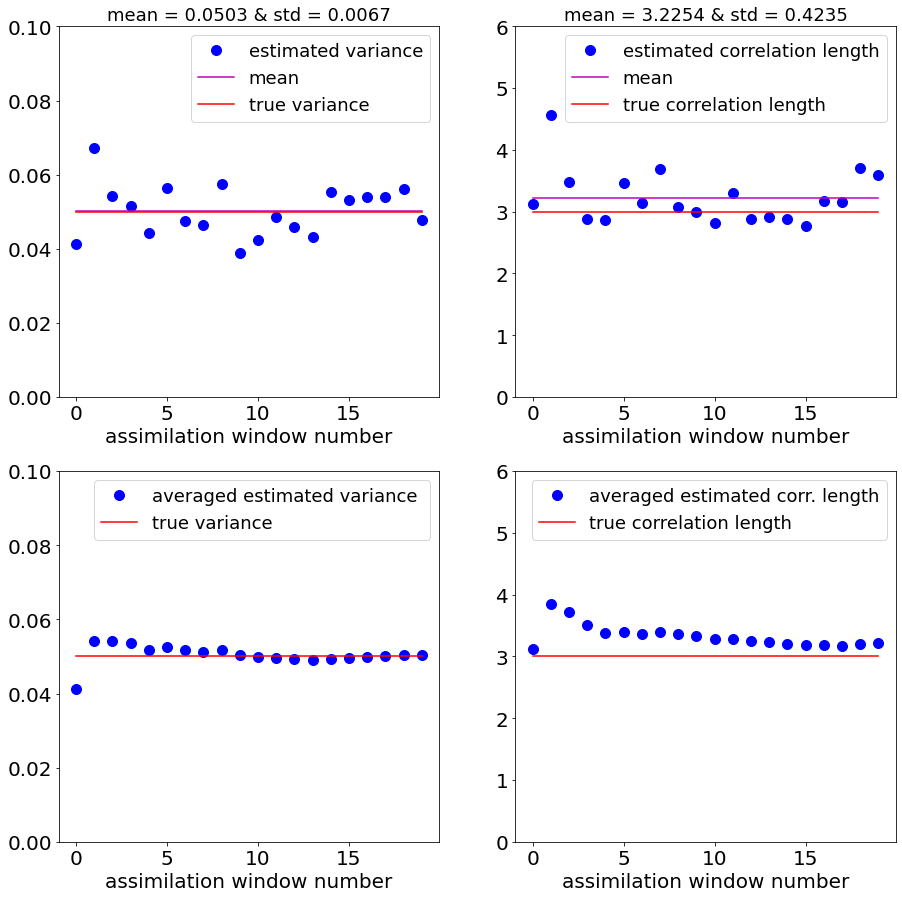
\includegraphics[scale=0.4]{Ex1}

%$[0.03013601 0.20059355 0.05104361 0.05340796 0.07825878 0.04791606 0.0351381  0.03679589 0.06804059 0.05433527 0.05633796 0.04327099 0.0359264  0.03473148 0.03984117 0.04640998 0.05816832 0.05292091 0.06412014 0.02973197]
%[3.0709382  6.84944213 3.24405428 4.08552994 5.06958417 2.55234062 3.17142044 2.89793485 3.08407158 6.06248414 4.04347102 2.69269948  2.55923644 3.01257032 2.04598122 3.30079194 2.30424979 3.45488984 5.07564751 2.8737259 ]$
\newpage
\subsubsection*{Experiment 2 - partial observation in space}
Same parameters as in Experiment 1, the only difference is that we observe only every second state variable, i.e. $m_x=100$ and $\Delta m_x=2$. 

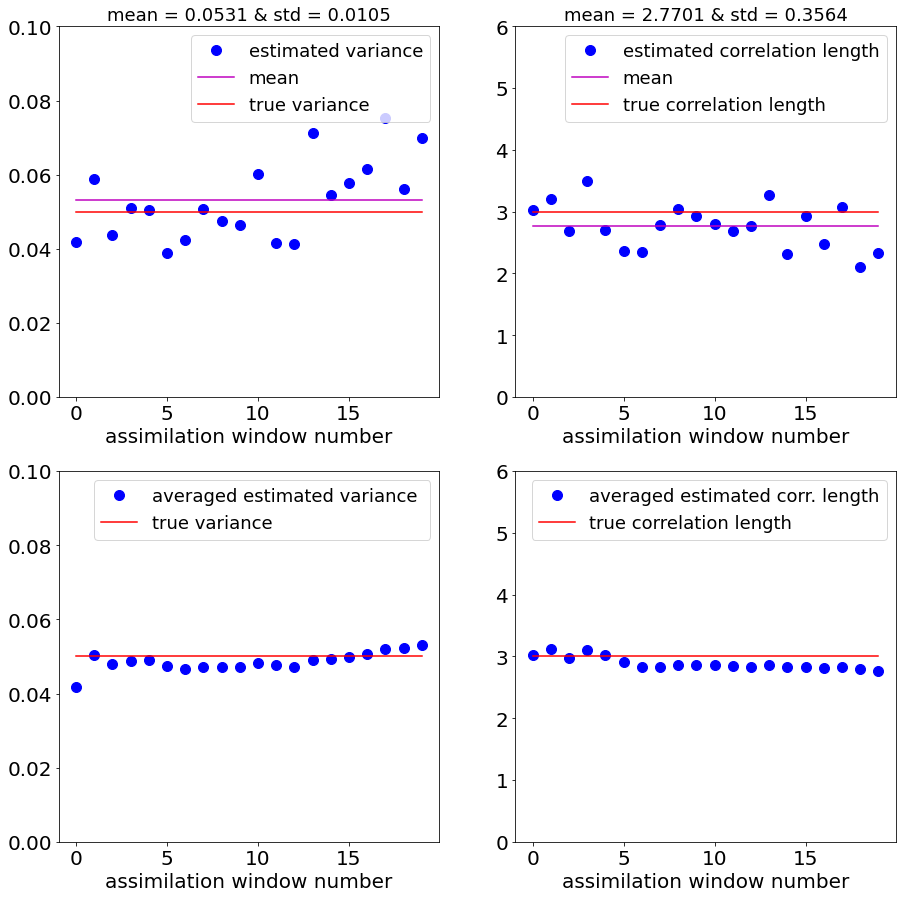
\includegraphics[scale=0.4]{Ex2}

\newpage
\subsubsection*{Experiment 3 - partial observation in time}
Same parameters as in Experiment 1, the only difference is that we observe only every second time step, i.e. $m_t=3$ and $\Delta m_t=2$.

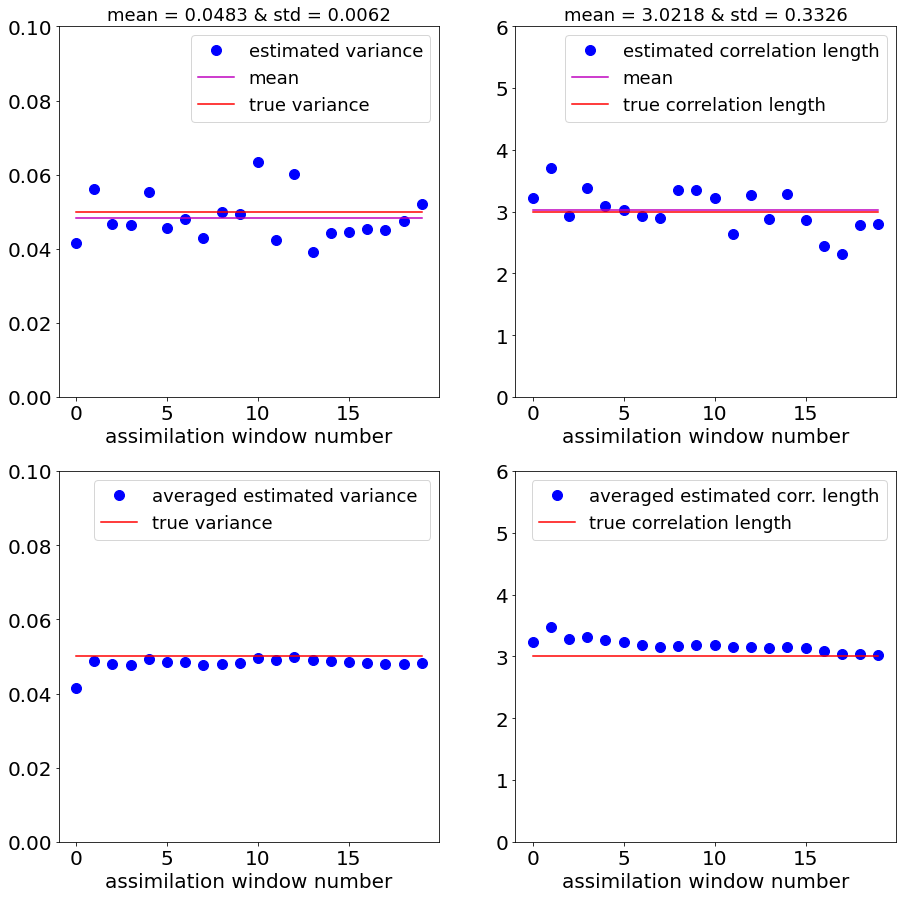
\includegraphics[scale=0.4]{Ex3}

\newpage
\subsubsection*{Experiment 4 - partial observation in time and space}
Same parameters as in Experiment 1, the only difference is that we observe only every second time step and every second time step, i.e. $m_t=3$ and $\Delta m_t=2$ and $m_x=100$ and $\Delta m_x=2$. 


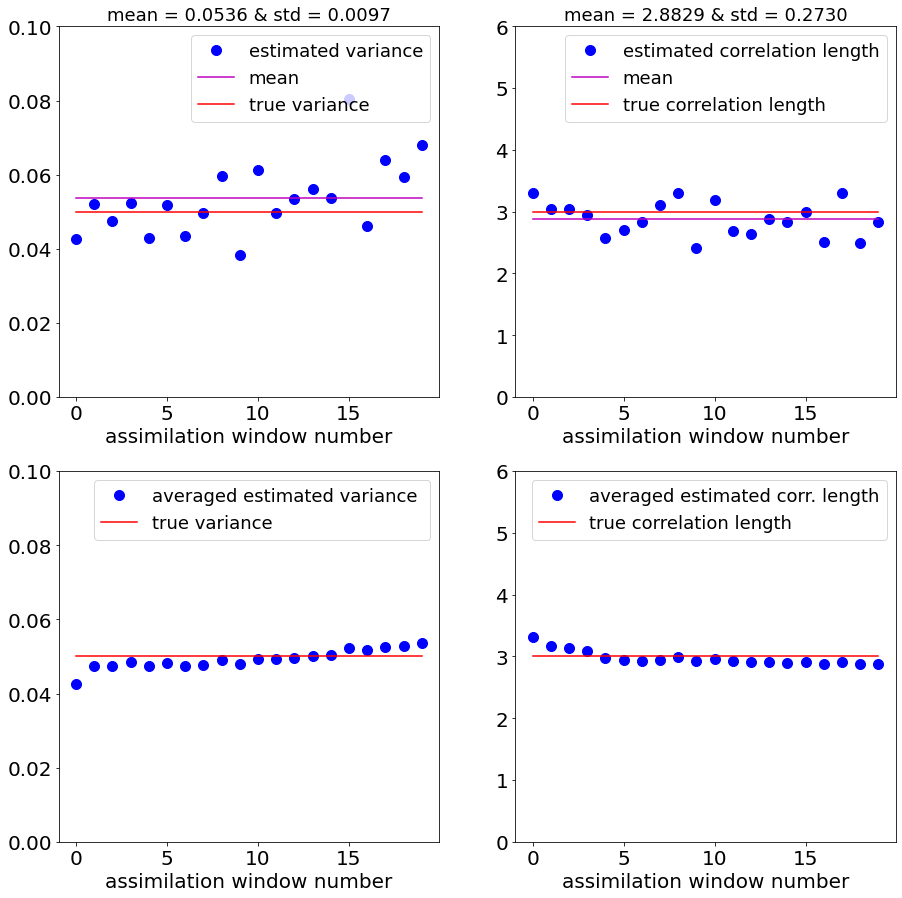
\includegraphics[scale=0.4]{Ex4}

\subsubsection*{Experiment 5 - partial observation in time and space, complicated $B$}
Same parameters as in Experiment 1, the only difference is that we observe only every second time step and every second time step, i.e. $m_t=3$ and $\Delta m_t=2$ and $m_x=100$ and $\Delta m_x=2$. Moreover, $\ell_t=5$ and we assume $B$ has variance $0.01$ and correlation length $3$ and we use this as our initial guess for $Q$. 

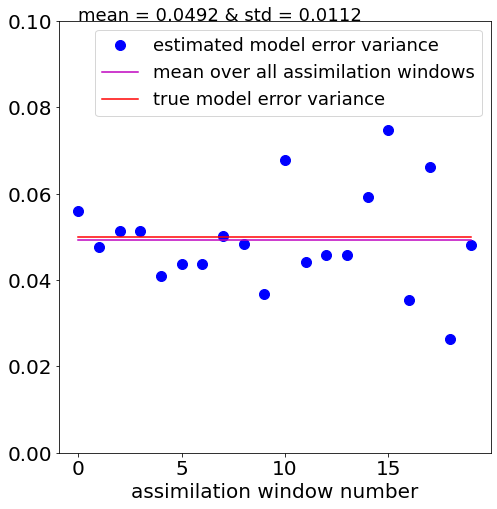
\includegraphics[scale=0.4]{Ex5var}
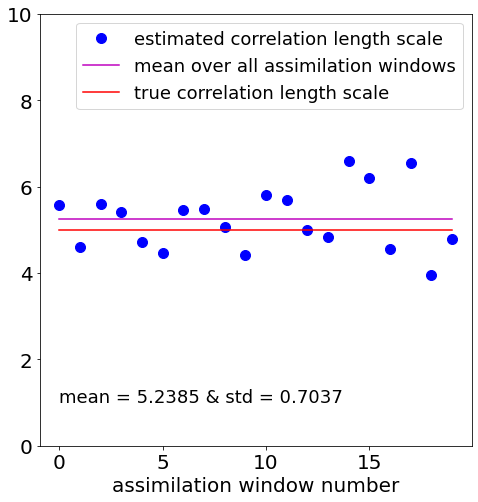
\includegraphics[scale=0.4]{Ex5len}\\
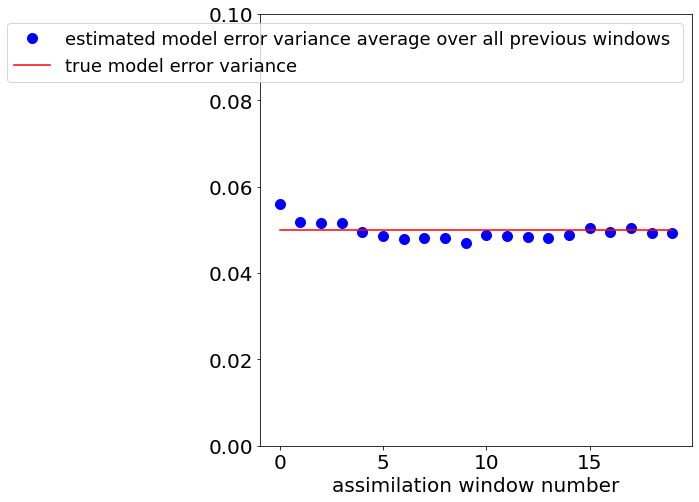
\includegraphics[scale=0.4]{Ex5meanvar}\hspace{-3cm}
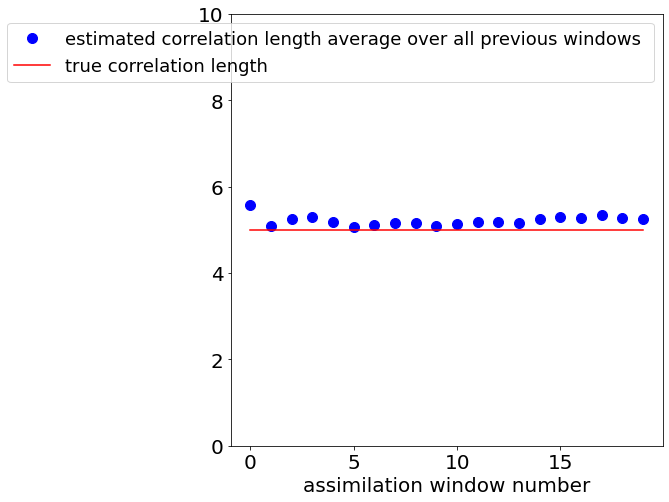
\includegraphics[scale=0.4]{Ex5meanlen}

\subsubsection*{Experiment 6 - partial observation in time and space, complicated $B$}
Same as experiment 5, only difference is that only every fourth gridpoint is observed. 

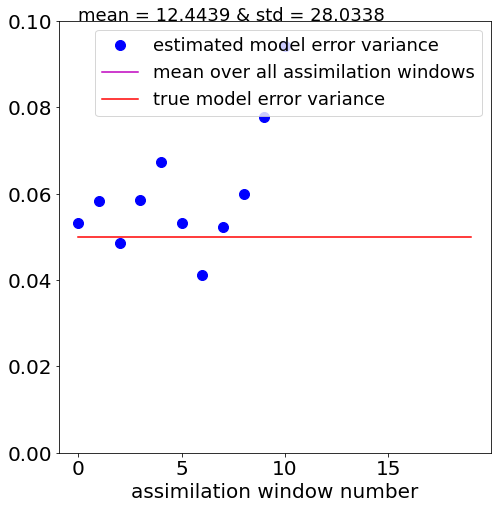
\includegraphics[scale=0.4]{Ex6var}
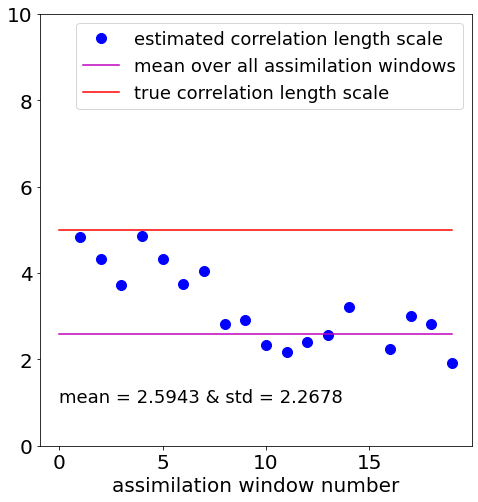
\includegraphics[scale=0.4]{Ex6len}\\
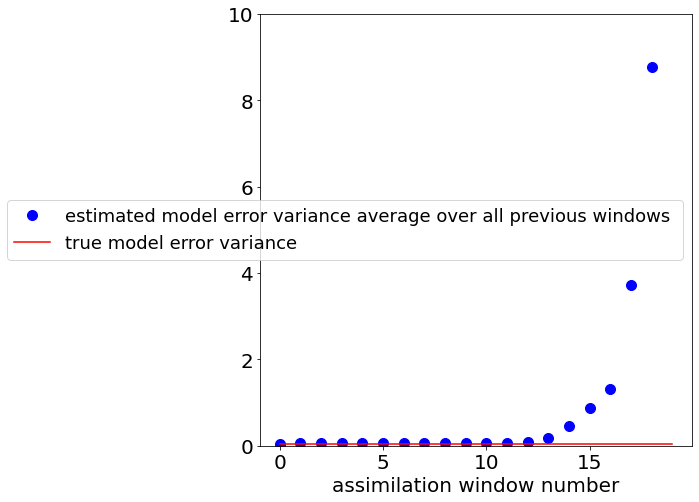
\includegraphics[scale=0.4]{Ex6meanvar}\hspace{-3cm}
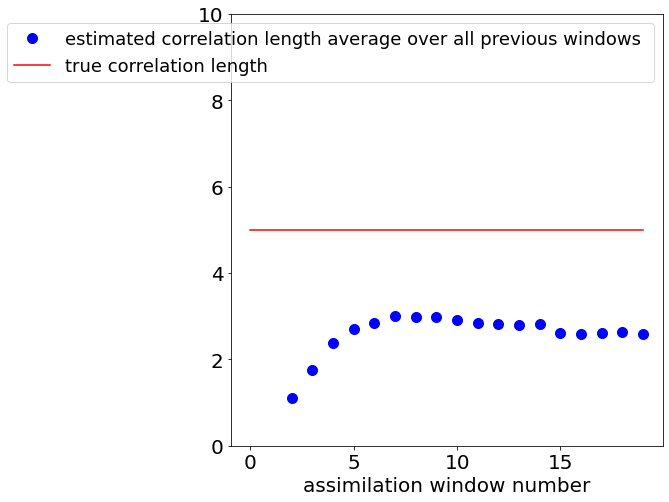
\includegraphics[scale=0.4]{Ex6meanlen}


\newpage
\section{Convergence proof}
\textcolor{red}{need to think about this}\\
It is surprisingly easy to proof convergence. Start with writing the prior estimate for $Q$ as
\begin{equation}
Q_0 = Q_t + E_0
\end{equation}
where we assume $\Vert E \Vert << \Vert Q_t \Vert$. Let's now write the Kalman gain used in the data assimilation as:
\begin{eqnarray}
K_0 & = & D_0H_z^T(H_zD_0H_z^T + R)^{-1} \nonumber \\
& = & (D_t + E_0)H_z^T(H_zD_0H_z^T + R +H_zE_0H_z^T )^{-1} \nonumber \\
& = & (D_t + E_0) H_z^T(H_zD_0H_z^T + R)^{-1}\left(I +H_zE_0H_z^T(H_zD_0H_z^T + R)^{-1} \right)^{-1}  \nonumber \\
& = & D_tH_z^T(H_zD_0H_z^T + R)^{-1}\left(I -H_zE_0H_z^T(H_zD_0H_z^T + R)^{-1} \right) + E_0H_z^T(H_zD_0H_z^T + R)^{-1}+O\left(\Vert E_0 \Vert^2 \right)  \nonumber \\
& = & K_t - K_t H_zE_0H_z^T(H_zD_0H_z^T + R)^{-1}  + E_0H_z^T(H_zD_0H_z^T + R)^{-1} + O\left(\Vert E_0 \Vert^2 \right) \nonumber \\
& = & K_t + (I-K_tH_z)K_E
\end{eqnarray}
in which
\begin{equation}
K_E = E_0H_z^T(H_zD_0H_z^T + R)^{-1}
\end{equation}
Let us now form
\begin{eqnarray}
<z_d c^T> & = & <K(y-H_x x_b)(y-H_x x_b)^T H_x>  \nonumber \\
& = & K(H_zDH_z^T + R)H_x^T \nonumber \\
& = & D_tH_z^TH_x + (I-K_t H_z)E_0H_z^T H_x
\end{eqnarray}
This has to be equal the the right-hand-side in our expression above, leading to:
\begin{equation}
D_tH_z^TH_x + (I-K_t H_z)E_0H_z^T H_x = (D_t + E_1)H_z^T H_x
\end{equation}
such that
\begin{equation}
E_1 H_z^T H_x = (I-K_t H_z)E_0H_z^T H_x 
\end{equation}
Since
\begin{eqnarray}
\Vert(I-K_t H_z)\Vert &  = & \Vert(I-(D^{-1}+H_z^TR^{-1}H_z)H_z^TR^{-1}H_z)\Vert \nonumber \\
& = & \Vert((D^{-1}+H_z^TR^{-1}H_z) (D^{-1}+H_z^TR^{-1}H_z - H_z^TR^{-1}H_z)\Vert \nonumber \\
& = &  \Vert((D^{-1}+H_z^TR^{-1}H_z) D^{-1}\Vert < 1
\end{eqnarray}
we see that $E_n$ convergence to zero when we iterate the scheme.

However, it is important to note that the $H_z^TH_x$ term projects on the observation space, so it might be that convergence is faster in the observed part than in the unobserved part of $D$, and hence of $Q$. Since we assume $Q$ to be the same in observed and unobserved parts of the domain we can smooth out this difference in convergence by averaging over observed and unobserved gridpoints simultaneously. But it might be that we cannot estimate $B$ with any accuracy (although $H_z^T = P^{-T}H_x$ might spread information to time zero via $P$). 

\newpage
\bibliography{lit.bib}{}
\bibliographystyle{plain}
\end{document}